\chapter{Surface Parameterization and Geometry}
\label{ch:surface_geometry}

\section{BFF Parameterization}
\label{sec:bff_parameterization}

\subsection{1. Overview}

Boundary First Flattening (BFF) is a state-of-the-art method for \index{conformal parameterization}\textbf{conformal parameterization} of surface meshes, introduced by Keenan Crane et al.\ in 2017\cite{crane2017}. Unlike traditional methods like Harmonic Mapping or LSCM, BFF allows the user to prescribe the target boundary curvature, providing unmatched control over the flattening process (e.g., flattening to a disk, a rectangle, or a specific shape).

\subsection{2. Definitions}

\begin{definition}[Conformal Mapping]\label{def:conformal_mapping}
A mapping that locally preserves angles between curves on a surface.
\end{definition}

\begin{definition}[Laplacian Matrix]\label{def:laplacian_matrix_bff}
A discrete representation of the Laplace-Beltrami operator, typically constructed using cotangent weights.
\end{definition}

\begin{definition}[Scale Factor]\label{def:scale_factor}
A scalar field $u$ on the mesh representing the local scaling needed to achieve the target metric under a conformal transformation $g' = e^{2u}g$.
\end{definition}

\begin{definition}[Geodesic Curvature]\label{def:geodesic_curvature_bff}
The curvature of a curve on a surface, relative to the surface itself.
\end{definition}

\subsection{3. Theory}

BFF is rooted in the \index{Yamabe equation}\textbf{Yamabe equation}, which describes how the metric changes under a conformal transformation $g' = e^{2u}g$\cite{crane2017}. The target geodesic curvature $\kappa'$ on the boundary relates to the original curvature $\kappa$ and the normal derivative of the scale factor $u$ by:
$$\kappa' = e^{-u}\left(\kappa + \frac{\partial u}{\partial n}\right)$$

BFF solves this by:
\begin{enumerate}
    \item Determining boundary scale factors $u$ that satisfy the target curvature $\kappa'$.
    \item Extending $u$ to the interior via a Dirichlet problem.
    \item Integrating the flattened boundary and extending the UV coordinates harmonically to the interior.
\end{enumerate}

\begin{example}[BFF Disk Flattening]\label{ex:bff_disk}
Consider a hemisphere mesh with a circular boundary. To flatten it to a disk, BFF sets the target geodesic curvature to $\kappa' = 2\pi/n$ at each of the $n$ boundary vertices (uniform curvature). The boundary system $L_{bb} \cdot u_b = \kappa' - \kappa$ is solved for the boundary scale factors, which encode how much each boundary edge must shrink or stretch. The interior scale factors are then determined by the Dirichlet problem, and the final UV coordinates are obtained by integrating the scaled edge lengths along the boundary and extending harmonically to the interior.
\end{example}

\subsection{4. Pseudocode}

\begin{algorithm}
\caption{BFF Parameterization}
\label{alg:bff_parameterization}
\begin{algorithmic}[1]
\Function{BFFParameterization}{$M$}
    \State Build the cotangent Laplacian matrix $L$ for mesh $M$
    \State Identify the boundary loop of $M$
    \State Compute the current geodesic curvature $\kappa$ at each boundary vertex
    \State Define the target curvature $\kappa_{\text{target}}$ (e.g., $2\pi/n$ for disk)
    \State Solve the boundary system for scale factors $u_b$: $L_{bb} \cdot u_b = \kappa_{\text{target}} - \kappa$
    \State Solve the Dirichlet problem for interior scale factors $u_i$: $L_{ii} \cdot u_i = -L_{ib} \cdot u_b$
    \State Integrate boundary coordinates $uv_b$ using $l_{\text{flat}} = l_{\text{orig}} \cdot \exp\left(\frac{u_i + u_j}{2}\right)$
    \State Extend $uv_b$ to the interior via harmonic mapping: $L_{ii} \cdot uv_i = -L_{ib} \cdot uv_b$
    \State \Return $UV$ coordinates for each vertex
\EndFunction
\end{algorithmic}
\end{algorithm}

\subsection{5. Parameter Selection}

\begin{itemize}
    \item \textbf{Target Curvature:} For a disk, set to $2\pi/n$. For a rectangle, set to $\pi/2$ at four vertices and $0$ elsewhere.
    \item \textbf{Solver:} Sparse direct solvers (like SuperLU) are recommended for solving the Laplacian systems.
\end{itemize}

\subsection{6. Complexity}

\begin{itemize}
    \item \textbf{Construction:} $O(N)$ for building the Laplacian.
    \item \textbf{Solving:} $O(N^{1.5})$ to $O(N^2)$ depending on mesh connectivity and sparse solver performance.
\end{itemize}

\subsection{7. Usages}

Implemented in \texttt{compgeom.mesh.surface.parameterization\_bff.BFFParameterizer}. Used for UV unwrapping, texture mapping, and surface remeshing.

\subsection{8. Testing Methods and Edge Cases}

\begin{itemize}
    \item \textbf{Testing:} Verify local angle preservation (conformal property). Check boundary curvature error.
    \item \textbf{Edge Cases:} Non-manifold meshes, meshes with no boundary (unsupported), and self-intersecting UV outputs.
\end{itemize}

\subsection{9. References}

\begin{itemize}
    \item Crane, K., Weischedel, C., \& Wardetzky, M. \cite{crane2017} ``Boundary first flattening.'' ACM TOG.
    \item Wikipedia: Conformal mapping.
\end{itemize}

\section{Harmonic Mapping}
\label{sec:harmonic_mapping}

\subsection{1. Overview}

Mesh Topology Transfer is the process of adapting a source mesh's connectivity (its faces and edges) to a new geometric boundary. This is achieved using \index{harmonic mapping}Harmonic Mapping, a technique that positions interior vertices to minimize a ``stretching'' energy (Dirichlet energy). The result is a new mesh that shares the same topology as the source but fits the geometry of the target domain with minimal distortion.

\subsection{2. Definitions}

\begin{definition}[Topology]\label{def:topology}
The connectivity of the mesh (which vertices form which faces), independent of their spatial coordinates.
\end{definition}

\begin{definition}[Harmonic Map]\label{def:harmonic_map}
A mapping between geometric domains that satisfies the Laplace equation $\Delta f = 0$.
\end{definition}

\begin{definition}[Barycentric Mapping]\label{def:barycentric_mapping}
A discrete version of harmonic mapping where every interior vertex is the weighted average of its neighbors.
\end{definition}

\begin{definition}[Dirichlet Energy]\label{def:dirichlet_energy}
A measure of how much a mapping ``stretches'' the domain; harmonic maps are the minimizers of this energy functional.
\end{definition}

\subsection{3. Theory}

Based on Tutte's Embedding Theorem\cite{tutte1963}, a valid planar embedding of a graph can be found by fixing its boundary to a convex polygon and solving for the interior positions such that each vertex is at the centroid of its neighbors.

\begin{theorem}[Tutte's Embedding Theorem]\label{thm:tutte}
Let $G$ be a planar graph with a distinguished boundary cycle mapped to a convex polygon. If every interior vertex is placed at the convex combination of its neighbors with strictly positive weights, the resulting embedding is a planar embedding with no edge crossings.
\end{theorem}

\begin{proof}
Tutte's proof\cite{tutte1963} uses a variational argument. The embedding minimizes the Dirichlet energy $E = \sum_{(i,j) \in E} w_{ij} \|p_i - p_j\|^2$ subject to the boundary constraints. Since the domain is convex and the weights are positive, the energy functional is strictly convex on the interior variables, guaranteeing a unique minimum. At the minimum, each interior vertex satisfies $\nabla_{p_i} E = 0$, which gives $p_i = \frac{1}{\sum_j w_{ij}} \sum_j w_{ij} p_j$---exactly the weighted average. The convexity of the target polygon, combined with the maximum principle for harmonic functions, ensures that no edge crossings occur.
\end{proof}

Mathematically, for each interior vertex $i$, we solve:
$$V_i = \frac{1}{\sum_{j \in N(i)} w_{ij}} \sum_{j \in N(i)} w_{ij} V_j$$

Where $w_{ij}$ are weights (often $w_{ij} = 1$ for simple barycentric mapping or cotangent weights for more accurate harmonic maps). This forms a system of linear equations $L V = B$, where $L$ is the Laplacian matrix and $B$ contains boundary constraints.

\begin{example}[Harmonic Mapping of a Square]\label{ex:harmonic_mapping}
Consider a $4 \times 4$ grid of vertices (a planar quad mesh) with the boundary vertices fixed to a unit square. Using uniform weights ($w_{ij} = 1$), each interior vertex is positioned at the arithmetic mean of its 4 neighbors. After convergence (typically 50--100 Gauss-Seidel iterations), the interior vertices distribute uniformly, producing a smooth parameterization of the square domain. This is the discrete harmonic map---the unique minimizer of the Dirichlet energy.
\end{example}

\subsection{4. Pseudocode}

\begin{algorithm}
\caption{Transfer Topology}
\label{alg:transfer_topology}
\begin{algorithmic}[1]
\Function{TransferTopology}{$source\_mesh, target\_boundary$}
    \State $source\_boundary \gets \text{GetBoundaryCycle}(source\_mesh)$
    \State $\text{MapBoundary}(source\_boundary, target\_boundary)$ \Comment{Using arc-length}
    \State $target\_centroid \gets \text{Centroid}(target\_boundary)$
    \For{$v \in \text{InteriorVertices}(source\_mesh)$}
        \State $v.\text{position} \gets target\_centroid$
    \EndFor
    \State $max\_delta \gets \infty$
    \While{$max\_delta > \epsilon$}
        \State $max\_delta \gets 0$
        \For{$v \in \text{InteriorVertices}(source\_mesh)$}
            \State $old\_pos \gets v.\text{position}$
            \State $neighbors \gets \text{GetNeighbors}(v, source\_mesh)$
            \State $v.\text{position} \gets \frac{\sum n.\text{position}}{|neighbors|}$
            \State $max\_delta \gets \max(max\_delta, \text{dist}(old\_pos, v.\text{position}))$
        \EndFor
    \EndWhile
    \State \Return $\text{CreateMesh}(new\_positions, source\_mesh.faces)$
\EndFunction
\end{algorithmic}
\end{algorithm}

\subsection{5. Parameter Selection}

\begin{itemize}
    \item \textbf{Iteration Count:} Typically 100--1000 iterations for the Gauss-Seidel solver, or use a direct sparse solver for large meshes.
    \item \textbf{Boundary Mapping:} Usually based on normalized arc-length to prevent the boundary vertices from ``bunching up'' in corners.
\end{itemize}

\subsection{6. Complexity}

\begin{itemize}
    \item \textbf{Time Complexity:} $O(n \cdot i)$ for the iterative solver (where $n$ is vertices, $i$ is iterations). $O(n \log n)$ or $O(n^{1.5})$ for direct sparse solvers.
    \item \textbf{Space Complexity:} $O(n + e)$ to store the mesh connectivity and vertex positions.
\end{itemize}

\subsection{7. Usages}

\begin{itemize}
    \item \textbf{Shape Morphing:} Smoothly transitioning one 3D model into another with the same topology.
    \item \textbf{Texture Mapping:} Unwrapping a 3D surface onto a 2D plane (UV mapping).
    \item \textbf{Remeshing:} Transferring a high-quality triangulation onto a newly defined boundary.
    \item \textbf{Surface Reconstruction:} Mapping a template mesh onto scanned point cloud data.
\end{itemize}

\subsection{8. Testing Methods and Edge Cases}

\begin{itemize}
    \item \textbf{Non-Convex Boundaries:} Tutte's theorem only guarantees no edge crossings for convex boundaries. For non-convex boundaries, self-intersections (flipped triangles) may occur.
    \item \textbf{Disconnected Components:} The algorithm must be applied to each connected component of the mesh separately.
    \item \textbf{High Valence Vertices:} Vertices with many neighbors may converge more slowly.
    \item \textbf{Meshes with Holes:} Requires mapping multiple boundary cycles (e.g., one to the outer boundary, others to internal ``islands'').
\end{itemize}

\subsection{9. References}

\begin{itemize}
    \item Tutte, W. T. \cite{tutte1963} ``How to draw a graph.'' Proceedings of the London Mathematical Society.
    \item Floater, M. S. (1997). ``Parametrization and smooth approximation of surface triangulations.'' Computer Aided Geometric Design.
    \item Pinkall, U., \& Polthier, K. (1993). ``Computing discrete minimal surfaces and their conjugates.'' Computing.
    \item Wikipedia: Tutte embedding.
\end{itemize}

\section{Functional Maps}
\label{sec:functional_maps}

\subsection{1. Overview}

\index{functional maps}Functional maps are a powerful framework for finding correspondences between 3D shapes\cite{ovsjanikov2012}. Instead of mapping points directly to points, which is a combinatorial problem, functional maps represent the correspondence as a linear operator between \textbf{functions} defined on the surfaces. This transformation from a point-based to a functional representation turns the non-convex matching problem into a much simpler linear algebra problem in a reduced basis.

\subsection{2. Definitions}

\begin{definition}[Basis Functions]\label{def:basis_functions_fm}
A set of smooth functions $\{\phi_i\}$ defined on a surface, typically the eigenfunctions of the Laplace-Beltrami operator.
\end{definition}

\begin{definition}[Functional Map]\label{def:functional_map}
A matrix $C$ that maps coefficients of a function in shape $A$'s basis to coefficients in shape $B$'s basis.
\end{definition}

\begin{definition}[Correspondence]\label{def:correspondence}
A mapping $\Pi$ from vertices of shape $A$ to vertices of shape $B$.
\end{definition}

\begin{definition}[Commutativity]\label{def:commutativity}
The property that a functional map should commute with other geometric operators (like the Laplacian), i.e., $C \Delta_A \approx \Delta_B C$.
\end{definition}

\subsection{3. Theory}

Given two shapes $M$ and $N$, we compute the first $k$ eigenfunctions of their respective Laplacians: $\Phi = [\phi_1, \dots, \phi_k]$ and $\Psi = [\psi_1, \dots, \psi_k]$. Any function $f$ on surface $M$ can be approximated as $f \approx \Phi \mathbf{a}$.

A correspondence between $M$ and $N$ can be represented by a matrix $C$ such that if $f$ is a function on $M$ and $g$ is its corresponding function on $N$, then $\mathbf{b} = C \mathbf{a}$, where $\mathbf{b}$ are the coefficients of $g$ in basis $\Psi$.

The matrix $C$ is found by solving an optimization problem:
$$\min_C \| C A - B \|^2 + \alpha \| C \Delta_M - \Delta_N C \|^2$$

where $A$ and $B$ are coefficients of ``descriptor functions'' (like curvature or HKS\cite{coifman2006}) that should be preserved under the mapping.

\begin{theorem}[Functional Map from Pointwise Map]\label{thm:fm_from_pointwise}
Given a pointwise correspondence $\Pi: M \to N$ between two shapes, the induced functional map is $C = \Psi^\dagger \Pi^\top \Phi$, where $\dagger$ denotes the pseudoinverse.
\end{theorem}

\begin{proof}
For a function $f$ on $M$ with coefficient vector $\mathbf{a} = \Phi^\dagger f$, the pullback $\Pi_* f = f \circ \Pi^{-1}$ has coefficients $\mathbf{b} = \Psi^\dagger (f \circ \Pi^{-1})$. Substituting $f = \Phi \mathbf{a}$, we get $\mathbf{b} = \Psi^\dagger \Pi^\top \Phi \mathbf{a}$, so $C = \Psi^\dagger \Pi^\top \Phi$.
\end{proof}

\begin{example}[Functional Map for Shape Matching]\label{ex:functional_map}
Consider two discretizations of a sphere (shapes $A$ and $B$) with a $90^\circ$ rotation between them. The first $k$ eigenfunctions of the Laplacian on both spheres are the spherical harmonics. The functional map $C$ corresponding to the rotation is a $k \times k$ block-diagonal matrix where each block is a rotation matrix acting on the harmonic subspace of a given frequency. With $k = 50$ basis functions, $C$ captures the rotation precisely, and the pointwise correspondence can be recovered by comparing the columns of $\Psi C$ with the columns of $\Phi$.
\end{example}

\subsection{4. Pseudocode}

\begin{algorithm}
\caption{Compute Functional Map}
\label{alg:compute_functional_map}
\begin{algorithmic}[1]
\Function{ComputeFunctionalMap}{$mesh\_A, mesh\_B, num\_basis=50$}
    \State $L_A, M_A \gets \text{ComputeLaplacianAndMass}(mesh\_A)$
    \State $L_B, M_B \gets \text{ComputeLaplacianAndMass}(mesh\_B)$
    \State $evals\_A, \Phi \gets \text{eigsh}(L_A, M_A, k=num\_basis)$
    \State $evals\_B, \Psi \gets \text{eigsh}(L_B, M_B, k=num\_basis)$
    \State $desc\_A \gets \text{ComputeHKS}(mesh\_A, \Phi, evals\_A)$
    \State $desc\_B \gets \text{ComputeHKS}(mesh\_B, \Psi, evals\_B)$
    \State $A\_coeffs \gets \Phi^\top \cdot M_A \cdot desc\_A$
    \State $B\_coeffs \gets \Psi^\top \cdot M_B \cdot desc\_B$
    \State $C \gets \text{SolveLeastSquares}(A\_coeffs^\top, B\_coeffs^\top)^\top$
    \State $C \gets \text{RefineMap}(C, \Phi, \Psi)$ \Comment{Optional ICP refinement}
    \State \Return $C$
\EndFunction
\end{algorithmic}
\end{algorithm}

\subsection{5. Parameter Selection}

\begin{itemize}
    \item \textbf{Number of Basis Functions ($k$):} Typically 30--100. More basis functions capture more detail but increase computation and noise sensitivity.
    \item \textbf{Descriptors:} High-quality descriptors (like HKS, WKS, or SHOT) are critical for a good initial map.
    \item \textbf{Regularization:} Weighting the Laplacian commutativity term helps ensure the map is ``smooth'' and ``geometric.''
\end{itemize}

\subsection{6. Complexity}

\begin{itemize}
    \item \textbf{Eigen-decomposition:} $O(N^{1.5})$ for sparse Laplacian matrices.
    \item \textbf{Map Calculation:} $O(k^3 + k^2 \cdot D)$ where $D$ is the number of descriptors.
    \item \textbf{Point Recovery:} $O(N \cdot k)$ using nearest neighbor search in the spectral embedding.
\end{itemize}

\subsection{7. Usages}

\begin{itemize}
    \item \textbf{Shape Matching:} Finding how one 3D character corresponds to another for animation transfer.
    \item \textbf{Statistical Shape Analysis:} Building a ``mean shape'' from a collection of scanned objects.
    \item \textbf{Texture Transfer:} Mapping a texture from one model to another with a different topology.
    \item \textbf{Symmetry Detection:} Finding self-correspondences within a single shape.
    \item \textbf{Shape Interpolation:} Generating intermediate shapes between two models.
\end{itemize}

\subsection{8. Testing Methods and Edge Cases}

\begin{itemize}
    \item \textbf{Identical Shapes:} The functional map $C$ should be an identity matrix.
    \item \textbf{Isometries:} For shapes that are bent but not stretched (like a human in different poses), $C$ should be nearly orthogonal ($C^\top C \approx I$).
    \item \textbf{Partial Matching:} Test how the algorithm handles shapes where parts are missing (requires more advanced ``Partial Functional Maps'' logic).
    \item \textbf{Topology Changes:} Verify that functional maps can still find a reasonable matching even if one shape has a different genus.
    \item \textbf{Low Resolution:} Ensure the basis is stable even on coarse meshes.
\end{itemize}

\subsection{9. References}

\begin{itemize}
    \item Ovsjanikov, M., Ben-Chen, M., Solomon, J., Butscher, A., \& Guibas, L. \cite{ovsjanikov2012} ``Functional maps: a flexible representation of maps between shapes.'' ACM TOG.
    \item Solomon, J., Nguyen, A., Butscher, A., Guibas, L., \& Ovsjanikov, M. (2016). ``Soft maps between surfaces.'' Computer Graphics Forum.
    \item Ovsjanikov, M., et al. (2017). ``Computing and Processing Correspondences with Functional Maps.'' SIGGRAPH Course.
    \item Wikipedia: Spectral shape analysis.
\end{itemize}

\section{Diffusion Distance}
\label{sec:diffusion_distance}

\index{diffusion distance}Diffusion distance is an intrinsic metric on a Riemannian manifold (or its discrete mesh representation) that measures the connectivity of points through a diffusion process\cite{coifman2006}.

\subsection{Overview}

Unlike Euclidean distance, which ignores the underlying shape, or \index{geodesic distance}Geodesic distance, which is sensitive to small topological changes (like ``short circuits''), diffusion distance is robust to noise and captures the global structure of the shape. It is based on the \index{heat kernel}Heat Kernel $K_t(x, y)$, which represents the probability of a random walker moving from $x$ to $y$ in time $t$.

The diffusion distance $d_t(x, y)$ is defined as:
$$d_t^2(x, y) = \int_M |K_t(x, u) - K_t(y, u)|^2 \, du$$

\begin{definition}[Diffusion Distance]\label{def:diffusion_distance}
Given a manifold $M$ and a time parameter $t > 0$, the diffusion distance between points $x, y \in M$ is $d_t(x,y) = \left(\int_M |K_t(x,u) - K_t(y,u)|^2 \, du\right)^{1/2}$, where $K_t$ is the heat kernel at time $t$.
\end{definition}

\subsection{Spectral Representation}

In the discrete setting, diffusion distance can be computed efficiently using the eigenvalues $\lambda_i$ and eigenvectors $\phi_i$ of the \index{Laplace-Beltrami operator}Laplace-Beltrami operator:
$$d_t^2(x, y) = \sum_{i=1}^k e^{-2\lambda_i t} (\phi_i(x) - \phi_i(y))^2$$

This allows for a \textbf{diffusion embedding} where each vertex $x$ is mapped to a point in $\mathbb{R}^k$:
$$\Psi_t(x) = \left(e^{-\lambda_1 t}\phi_1(x),\; e^{-\lambda_2 t}\phi_2(x),\; \dots,\; e^{-\lambda_k t}\phi_k(x)\right)$$

The Euclidean distance in this embedding space is exactly the diffusion distance.

\subsection{Usage}

\begin{algorithm}
\caption{Compute Diffusion Distance}
\label{alg:compute_diffusion_distance}
\begin{algorithmic}[1]
\Function{ComputeDiffusionDistance}{$mesh, i, j, t$}
    \State Compute eigenvalues $\lambda$ and eigenvectors $\phi$ of the Laplace-Beltrami operator
    \State $d^2 \gets \sum_{k} e^{-2\lambda_k t} (\phi_k(i) - \phi_k(j))^2$
    \State \Return $\sqrt{d^2}$
\EndFunction
\\
\Function{ComputeDiffusionEmbedding}{$mesh, t, k$}
    \State Compute eigenvalues $\lambda$ and eigenvectors $\phi$ of the Laplace-Beltrami operator
    \For{each vertex $x$}
        \State $\Psi_t(x) \gets \left(e^{-\lambda_1 t}\phi_1(x), \dots, e^{-\lambda_k t}\phi_k(x)\right)$
    \EndFor
    \State \Return $\Psi_t$
\EndFunction
\end{algorithmic}
\end{algorithm}

\subsection{References}

\begin{itemize}
    \item Coifman, R. R., \& Lafon, S. \cite{coifman2006} ``Diffusion maps.'' Applied and Computational Harmonic Analysis.
    \item Bronstein, A. M., et al. ``Numerical Geometry of Non-Rigid Shapes.'' Springer, 2008.
\end{itemize}

\section{Mean Curvature Flow}
\label{sec:mean_curvature_flow}

\subsection{1. Overview}

Polygonal \index{mean curvature flow}Mean Curvature Flow is a geometric process used to smooth the boundaries of a polygon\cite{gage1986,grayson1987}. It is a discrete version of the curve-shortening flow, where each point on a curve moves in the direction of its curvature vector. Over time, this process eliminates high-frequency noise and sharp corners, causing the polygon to become smoother and more circular.

\subsection{2. Definitions}

\begin{definition}[Mean Curvature (Curves)]\label{def:mean_curvature_curve}
In the context of curves, this is the rate at which the tangent direction changes along the curve, i.e., $\kappa = \frac{d\theta}{ds}$ where $\theta$ is the tangent angle and $s$ is arc length.
\end{definition}

\begin{definition}[Discrete Laplacian]\label{def:discrete_laplacian}
An operator that approximates the second derivative of the vertex positions. For a vertex $V_i$ in a polygon, $L_i = V_{i-1} - 2V_i + V_{i+1}$.
\end{definition}

\begin{definition}[Time Step]\label{def:time_step_mcf}
A parameter $\Delta t$ controlling the magnitude of displacement in each iteration. Must satisfy $\Delta t < 0.5$ for numerical stability.
\end{definition}

\subsection{3. Theory}

The flow is based on the diffusion equation (heat equation) applied to geometry: $\frac{\partial P}{\partial t} = \Delta P$. In a discrete polygon, moving a vertex $V_i$ by its Laplacian is equivalent to moving it toward the midpoint of its two neighbors ($V_{i-1}$ and $V_{i+1}$). This local averaging effect reduces the ``sharpness'' of vertices.

\begin{theorem}[Gage--Hamilton--Grayson Theorem]\label{thm:gage_hamilton_grayson}
Any simple closed plane curve evolving under curve-shortening flow (mean curvature flow) becomes convex in finite time and subsequently shrinks to a round point.
\end{theorem}

\begin{proof}
The proof proceeds in two stages. Gage and Hamilton (1986)\cite{gage1986} showed that any simple closed curve with non-negative curvature evolves to become convex. Grayson (1987)\cite{grayson1987} completed the argument by showing that if a curve is not initially convex, the flow eventually makes it convex, after which the Gage--Hamilton result applies. The key ingredient is the monotonicity of the width of the curve under the flow and the maximum principle applied to the curvature.
\end{proof}

A known property of this flow is that any simple closed curve will eventually become convex and then shrink to a circular point. To use this for smoothing without losing the shape entirely, the process is usually limited to a few iterations or includes a scaling step to preserve the original perimeter or area.

\begin{example}[Mean Curvature Flow on a Star Shape]\label{ex:mcf_star}
Consider a 5-pointed star polygon with 10 vertices (5 tips, 5 valleys). At each iteration with $\Delta t = 0.1$:
\begin{itemize}
    \item \textbf{Step 0}: The tips have large negative curvature (sharp outward corners) and the valleys have large positive curvature.
    \item \textbf{Step 1}: Tips move inward (toward midpoints of their neighbors), valleys move outward. The star becomes less pointy.
    \item \textbf{Step 5}: The polygon is noticeably smoother. The concavities are reduced.
    \item \textbf{Step 20}: The polygon is nearly convex and approximately elliptical.
\end{itemize}
After enough iterations (without size preservation), it would shrink to a point. With perimeter preservation, it converges to a smooth, near-circular shape.
\end{example}

\subsection{4. Pseudocode}

\begin{algorithm}
\caption{Mean Curvature Flow}
\label{alg:mean_curvature_flow}
\begin{algorithmic}[1]
\Function{MeanCurvatureFlow}{$polygon, iterations, dt, preserve\_size$}
    \State $n \gets \text{len}(polygon)$
    \State $current \gets polygon$
    \State $original\_perimeter \gets \text{CalculatePerimeter}(polygon)$
    \For{$k = 1$ \textbf{to} $iterations$}
        \State $next\_gen \gets []$
        \For{$i = 0$ \textbf{to} $n - 1$}
            \State $L_x \gets current[i{-}1].x - 2 \cdot current[i].x + current[i{+}1].x$
            \State $L_y \gets current[i{-}1].y - 2 \cdot current[i].y + current[i{+}1].y$
            \State $new\_x \gets current[i].x + dt \cdot L_x$
            \State $new\_y \gets current[i].y + dt \cdot L_y$
            \State $\text{append}(next\_gen, \text{Point}(new\_x, new\_y))$
        \EndFor
        \If{$preserve\_size$}
            \State $current\_perimeter \gets \text{CalculatePerimeter}(next\_gen)$
            \State $scale \gets original\_perimeter \;/\; current\_perimeter$
            \State $next\_gen \gets \text{Scale}(next\_gen, scale)$
        \EndIf
        \State $current \gets next\_gen$
    \EndFor
    \State \Return $current$
\EndFunction
\end{algorithmic}
\end{algorithm}

\subsection{5. Parameter Selection}

\begin{itemize}
    \item \textbf{Time Step ($\Delta t$):} Typically set between 0.01 and 0.2. Values above 0.5 can lead to numerical instability where the polygon ``explodes.''
    \item \textbf{Iterations:} Depends on the level of noise. Usually 10--100 steps are sufficient for smoothing.
    \item \textbf{Preservation:} \texttt{keep\_perimeter} or \texttt{keep\_area} prevents the polygon from shrinking to a point.
\end{itemize}

\subsection{6. Complexity}

\begin{itemize}
    \item \textbf{Time Complexity:} $O(n \cdot i)$, where $n$ is the number of vertices and $i$ is the number of iterations.
    \item \textbf{Space Complexity:} $O(n)$ to store the vertex positions.
\end{itemize}

\subsection{7. Usages}

\begin{itemize}
    \item \textbf{Image Processing:} Smoothing the results of contour extraction.
    \item \textbf{GIS:} Generalizing map boundaries for different zoom levels.
    \item \textbf{Computer Graphics:} Creating organic-looking shapes from blocky initial geometry.
    \item \textbf{CAD:} Removing artifacts from digitized or scanned blueprints.
\end{itemize}

\subsection{8. Testing Methods and Edge Cases}

\begin{itemize}
    \item \textbf{Jagged Input:} Verify that ``zig-zag'' patterns are flattened.
    \item \textbf{Stability:} Test with large $\Delta t$ to identify the breaking point.
    \item \textbf{Self-intersection:} Check if the flow resolves or creates new self-intersections.
    \item \textbf{Collinear Vertices:} Verify that straight edges remain straight.
    \item \textbf{Drift:} Ensure the centroid remains relatively stationary if re-centering is applied.
\end{itemize}

\subsection{9. References}

\begin{itemize}
    \item Gage, M., \& Hamilton, R. S. \cite{gage1986} ``The heat equation shrinking convex plane curves.'' Journal of Differential Geometry.
    \item Grayson, M. A. \cite{grayson1987} ``The heat equation shrinks embedded plane curves to round points.'' Journal of Differential Geometry.
    \item Desbrun, M., Meyer, M., Schr\"{o}der, P., \& Barr, A. H. (1999). ``Implicit fairing of irregular meshes using diffusion and curvature flow.'' SIGGRAPH.
    \item Wikipedia: Curve-shortening flow.
\end{itemize}

\section{Angle-Bounded Remeshing}
\label{sec:angle_bounded_remesher}

\index{angle-bounded remeshing}Angle-bounded remeshing is a surface mesh refinement process that improves the quality of a triangular mesh by enforcing specific bounds on the internal angles of all triangles.

\subsection{Overview}

High-quality triangular meshes are essential for accurate physical simulations\cite{botsch2010}. Small or large angles can lead to numerical instability. This remeshing technique (inspired by TriWild) iteratively modifies the mesh topology and geometry to improve the overall quality, targeting a minimum angle of $30^\circ$ and a maximum angle of $120^\circ$.

\subsection{Implementation Details}

The \texttt{AngleBoundedRemesher} in \texttt{CompGeom} uses a sequence of local mesh operations:
\begin{enumerate}
    \item \textbf{Edge Splits:} Long edges are split to reduce triangle size.
    \item \textbf{Edge Collapses:} Short edges are collapsed to remove small or sliver triangles.
    \item \textbf{Edge Flips:} Edges are flipped to maximize the minimum angle in the local quadrilateral.
    \item \textbf{Vertex Smoothing:} Vertices are moved to their local centroids (Laplacian smoothing) to create more uniform distributions.
\end{enumerate}

\subsection{Usage}

\begin{algorithm}
\caption{Angle-Bounded Remesh}
\label{alg:angle_bounded_remesh}
\begin{algorithmic}[1]
\Function{AngleBoundedRemesh}{$mesh, min\_angle, max\_angle, iterations$}
    \For{$k = 1$ \textbf{to} $iterations$}
        \State $\text{SplitLongEdges}(mesh, max\_angle)$
        \State $\text{CollapseShortEdges}(mesh, min\_angle)$
        \State $\text{FlipEdges}(mesh, min\_angle, max\_angle)$
        \State $\text{SmoothVertices}(mesh)$
    \EndFor
    \State \Return $mesh$
\EndFunction
\end{algorithmic}
\end{algorithm}

\subsection{References}

\begin{itemize}
    \item Hu, Y., et al. ``TriWild: Robust Remeshing with Angle Bounds.'' ACM Transactions on Graphics (SIGGRAPH), 2021.
    \item Botsch, M., et al. ``Polygon Mesh Processing.'' CRC Press, 2010.
\end{itemize}

\section{Affine Heat Flow}
\label{sec:affine_heat_flow}

\subsection{1. Overview}

\index{affine heat flow}Affine heat flow is a geometric smoothing process for polygons and curves that is invariant under affine transformations (rotation, scaling, translation, and shearing). While standard heat flow (curve shortening flow) tends to evolve shapes toward circles, affine heat flow evolves them toward ellipses. It is used in image processing and computer vision for shape simplification and denoising where the affine structure of the object must be preserved.

\subsection{2. Definitions}

\begin{definition}[Affine Invariance]\label{def:affine_invariance}
A property where the result of the flow on a transformed shape is the same as the transformation applied to the flow result.
\end{definition}

\begin{definition}[Euclidean Curvature]\label{def:euclidean_curvature}
The standard rate of change of the tangent direction: $\kappa = d\theta/ds$.
\end{definition}

\begin{definition}[Affine Curvature]\label{def:affine_curvature}
A measure of curvature that remains unchanged under affine maps, defined as $\kappa_a = \kappa^{1/3}$ for planar curves.
\end{definition}

\subsection{3. Theory}

Standard curve shortening flow is defined by $\frac{\partial P}{\partial t} = \kappa \mathbf{N}$.

Affine heat flow is defined by $\frac{\partial P}{\partial t} = \kappa^{1/3} \mathbf{N}$.

This specific power of $1/3$ is what provides the affine invariance. In the discrete case (for polygons), the flow is often implemented by iteratively updating vertex positions using a weighted average of their neighbors, but with weights that account for the local area or affine metric.

A common discrete approximation for a vertex $V_i$ with neighbors $V_{i-1}$ and $V_{i+1}$ is:
$$V_i^{\text{new}} = V_i + \Delta t \cdot \text{Area}(V_{i-1}, V_i, V_{i+1})^{1/3} \cdot \mathbf{N}_i$$

where $\mathbf{N}_i$ is the discrete normal vector.

\begin{example}[Affine Heat Flow on a Sheared Square]\label{ex:affine_heat}
Consider a square with vertices $(0,0), (1,0), (1,1), (0,1)$ that is sheared by the transformation $(x,y) \mapsto (x + 0.5y, y)$, giving vertices $(0,0), (1,0), (1.5,1), (0.5,1)$. Under standard curve-shortening flow, this shape would evolve toward a circle. Under affine heat flow, it evolves toward an ellipse whose eccentricity matches the affine structure of the original sheared square. If we then ``un-shear'' the result, we recover the same shape as applying affine heat flow directly to the original square.
\end{example}

\subsection{4. Pseudocode}

\begin{algorithm}
\caption{Affine Polygon Smoothing}
\label{alg:affine_polygon_smoothing}
\begin{algorithmic}[1]
\Function{AffinePolygonSmoothing}{$polygon, dt, iterations$}
    \State $current\_vertices \gets polygon.\text{vertices}$
    \For{$\_ = 1$ \textbf{to} $iterations$}
        \State $new\_vertices \gets []$
        \State $n \gets \text{len}(current\_vertices)$
        \For{$i = 0$ \textbf{to} $n - 1$}
            \State $v_{\text{prev}} \gets current\_vertices[(i - 1) \bmod n]$
            \State $v_{\text{curr}} \gets current\_vertices[i]$
            \State $v_{\text{next}} \gets current\_vertices[(i + 1) \bmod n]$
            \State $edge1 \gets v_{\text{curr}} - v_{\text{prev}}$
            \State $edge2 \gets v_{\text{next}} - v_{\text{curr}}$
            \State $area \gets 0.5 \cdot |\text{cross\_product}(edge1, edge2)|$
            \State $normal \gets \text{Normalize}\left(\text{Perpendicular}(edge2) + \text{Perpendicular}(edge1)\right)$
            \State $displacement \gets area^{1/3} \cdot normal \cdot dt$
            \State $\text{append}(new\_vertices, v_{\text{curr}} + displacement)$
        \EndFor
        \State $current\_vertices \gets new\_vertices$
    \EndFor
    \State \Return $\text{Polygon}(current\_vertices)$
\EndFunction
\end{algorithmic}
\end{algorithm}

\subsection{5. Parameter Selection}

\begin{itemize}
    \item \textbf{Time Step ($dt$):} Must be small enough to ensure stability (CFL condition).
    \item \textbf{Iterations:} More iterations result in smoother, more simplified shapes.
    \item \textbf{Area Threshold:} Small areas (near-collinear vertices) can lead to numerical instability; an epsilon threshold is often used.
\end{itemize}

\subsection{6. Complexity}

\begin{itemize}
    \item \textbf{Time Complexity:} $O(I \cdot n)$ where $I$ is iterations and $n$ is vertex count.
    \item \textbf{Space Complexity:} $O(n)$ to store the vertex positions.
\end{itemize}

\subsection{7. Usages}

\begin{itemize}
    \item \textbf{Shape Recognition:} Normalizing shapes to a ``canonical'' form before matching in a database.
    \item \textbf{Computer Vision:} Preprocessing object silhouettes to remove pixelation or noise while preserving geometric structure.
    \item \textbf{Cartography:} Simplifying coastlines or boundaries for small-scale maps.
    \item \textbf{Generative Design:} Creating organic, smooth shapes from rough polyline sketches.
    \item \textbf{Image Analysis:} Analyzing the ``affine scale space'' of an image.
\end{itemize}

\subsection{8. Testing Methods and Edge Cases}

\begin{itemize}
    \item \textbf{Ellipses:} An ellipse should remain an ellipse under affine heat flow (only its size should change).
    \item \textbf{Squares:} A square should gradually round its corners and evolve toward an ellipse.
    \item \textbf{Affine Symmetry:} Verify that shearing a polygon, smoothing it, and then ``un-shearing'' it gives the same result as smoothing the original polygon.
    \item \textbf{Self-Intersections:} Ensure the flow doesn't cause the polygon to cross itself (though this is theoretically possible for non-convex shapes).
    \item \textbf{Zero Area:} Handle perfectly collinear triplets of vertices.
\end{itemize}

\subsection{9. References}

\begin{itemize}
    \item Sapiro, G., \& Tannenbaum, A. (1993). ``Affine invariant scale-space.'' International Journal of Computer Vision.
    \item Olver, P. J., Sapiro, G., \& Tannenbaum, A. (1994). ``Affine invariant geometric evolutions of planar curves.'' SIAM Journal on Applied Mathematics.
    \item Angenent, S., Sapiro, G., \& Tannenbaum, A. (1998). ``On the affine heat equation for non-convex curves.'' Journal of the American Mathematical Society.
    \item Wikipedia: Affine shape adaptation.
\end{itemize}

\section{Geodesic Distance}
\label{sec:geodesic_distance}

\subsection{1. Overview}

Finding the shortest path between two points on a 3D surface mesh (the \index{geodesic distance}geodesic distance) is a fundamental problem in geometric modeling\cite{mitchell1987,crane2013geodesic,sethian1996}. Unlike Euclidean distance, which ignores the surface, the geodesic distance must follow the ``terrain'' of the mesh. While the Fast Marching Method (FMM) is the most famous numerical approach, other algorithms like the MMP algorithm (exact) and the Heat Method (highly efficient) provide different trade-offs between speed and accuracy.

\subsection{2. Definitions}

\begin{definition}[Geodesic]\label{def:geodesic}
The shortest path between two points on a surface, restricted to stay on that surface.
\end{definition}

\begin{definition}[MMP Algorithm]\label{def:mmp_algorithm}
An exact algorithm (Mitchell, Mount, Papadimitriou\cite{mitchell1987}) that generalizes Dijkstra's algorithm to continuous surfaces by propagating ``windows'' along edges.
\end{definition}

\begin{definition}[Heat Method]\label{def:heat_method}
A modern method (Crane et al.\ \cite{crane2013geodesic}) that approximates geodesics by observing the flow of heat from a source point.
\end{definition}

\begin{definition}[Edge-Walking]\label{def:edge_walking}
A simple approximation that treats the mesh as a graph and uses Dijkstra's algorithm on edges, which usually provides poor results as it cannot ``cut'' across faces.
\end{definition}

\subsection{3. Theory}

\subsubsection{MMP Algorithm (Exact)}

The MMP algorithm (Mitchell, Mount, and Papadimitriou\cite{mitchell1987}) works by propagating ``intervals'' of potential paths across the surface. When a wavefront reaches an edge, it creates a new set of intervals for the next triangle. This results in an exact polyhedral geodesic but is mathematically complex to implement.

\subsubsection{The Heat Method (Fast Approximation)}

The Heat Method\cite{crane2013geodesic}, introduced by Keenan Crane et al.\ (2013), uses a three-step process based on the heat equation:
\begin{enumerate}
    \item \textbf{Heat Flow:} Solve the heat equation $\dot{u} = \Delta u$ for a short time $t$, with a source at the starting vertex.
    \item \textbf{Gradient Normalization:} Calculate the gradient of the heat field $\nabla u$ and normalize it to have unit length ($X = -\nabla u / |\nabla u|$).
    \item \textbf{Poisson Solve:} Solve the Poisson equation $\Delta \phi = \nabla \cdot X$. The resulting scalar field $\phi$ is the geodesic distance to the source.
\end{enumerate}

\begin{figure}[htbp]
\centering
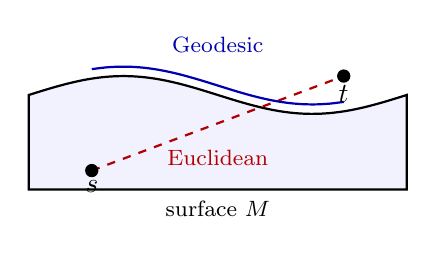
\begin{tikzpicture}[scale=0.8]
  \draw[thick,fill=blue!5] plot[smooth,domain=0:6,samples=40] (\x,{0.3*sin(\x*60)+1.5}) -- (6,0) -- (0,0) -- cycle;
  \draw[red!70!black,thick,dashed] (1,0.3) -- (5,1.8);
  \node[red!70!black,font=\footnotesize] at (3,0.5) {Euclidean};
  \draw[blue!70!black,thick] plot[smooth,domain=1:5,samples=20] (\x,{0.3*sin(\x*60)+1.5+0.15});
  \node[blue!70!black,font=\footnotesize] at (3,2.3) {Geodesic};
  \fill (1,0.3) circle (3pt) node[below] {$s$};
  \fill (5,1.8) circle (3pt) node[below] {$t$};
  \node[font=\footnotesize] at (3,-0.3) {surface $M$};
\end{tikzpicture}
\caption{Geodesic vs.\ Euclidean distance on a curved surface. The geodesic (blue) follows the terrain.}
\label{fig:geodesic}
\end{figure}


\begin{example}[Geodesic on a Cylinder]\label{ex:geodesic_cylinder}
Consider a cylinder of radius $r$ and height $h$. The geodesic between two points on opposite sides of the cylinder does not travel ``through'' the cylinder but wraps around it. If the two points are at the same height but separated by angle $\pi$ (opposite sides), the geodesic distance is $\pi r$ (half the circumference), not $2r$ (the Euclidean distance through the interior). The Heat Method computes this by solving the heat equation with a point source, normalizing the gradient, and solving a Poisson equation.
\end{example}

\subsection{4. Pseudocode}

\subsubsection{Heat Method}

\begin{algorithm}
\caption{Compute Geodesic via Heat Method}
\label{alg:compute_geodesic_heat}
\begin{algorithmic}[1]
\Function{ComputeGeodesicHeat}{$mesh, source\_vertex$}
    \State $L \gets \text{ComputeCotangentLaplacian}(mesh)$
    \State $A \gets \text{ComputeVertexAreas}(mesh)$
    \State $t \gets \text{mean\_edge\_length}(mesh)^2$
    \State $u \gets \text{SolveLinearSystem}(A - t \cdot L, source\_indicator)$
    \State $X \gets []$
    \For{$face \in mesh.\text{faces}$}
        \State $grad\_u \gets \text{ComputeFaceGradient}(face, u)$
        \State $\text{append}(X, -grad\_u \;/\; \text{norm}(grad\_u))$
    \EndFor
    \State $div\_X \gets \text{ComputeDivergence}(X, mesh)$
    \State $\phi \gets \text{SolveLinearSystem}(L, div\_X)$
    \State \Return $\phi - \phi[source\_vertex]$ \Comment{Shift so source is 0}
\EndFunction
\end{algorithmic}
\end{algorithm}

\subsection{5. Parameter Selection}

\begin{itemize}
    \item \textbf{Time Step ($t$):} In the Heat Method, $t$ is typically set to the square of the average edge length. Too small $t$ leads to numerical noise; too large $t$ leads to smoothing errors.
    \item \textbf{Solver:} Sparse direct solvers (like SuperLU or CHOLMOD) are essential for the Laplacian systems.
\end{itemize}

\subsection{6. Complexity}

\begin{itemize}
    \item \textbf{MMP Algorithm:} $O(n^2)$ in the worst case, but $O(n \log n)$ in practice.
    \item \textbf{Heat Method:} $O(n)$ after an initial $O(n^{1.5})$ matrix factorization. Subsequent queries from different sources are extremely fast.
\end{itemize}

\subsection{7. Usages}

\begin{itemize}
    \item \textbf{Surface Parameterization:} Normalizing distances for texture mapping.
    \item \textbf{Mesh Segmentation:} Grouping vertices based on their distance from a set of ``seeds.''
    \item \textbf{Shape Matching:} Using geodesic ``fingerprints'' to compare 3D models.
    \item \textbf{Texture Synthesis:} Propagation of patterns along a surface.
    \item \textbf{Medicine:} Measuring distances along the folds of the brain or surface of an organ.
\end{itemize}

\subsection{8. Testing Methods and Edge Cases}

\begin{itemize}
    \item \textbf{Flat Mesh:} The results should match the Euclidean distance exactly.
    \item \textbf{Sphere:} Geodesics between any two points should follow ``Great Circles.''
    \item \textbf{Concave Regions:} Verify that the path correctly ``bends'' into valleys rather than jumping across them.
    \item \textbf{Mesh Resolution:} Test how the accuracy of the Heat Method improves as the mesh is refined.
    \item \textbf{Boundaries:} Ensure the algorithm handles the edges of a surface without ``leaking'' or crashing.
\end{itemize}

\subsection{9. References}

\begin{itemize}
    \item Mitchell, J. S. B., Mount, D. M., \& Papadimitriou, C. H. \cite{mitchell1987} ``The discrete geodesic problem.'' SIAM Journal on Computing.
    \item Crane, K., Weischedel, C., \& Wardetzky, M. \cite{crane2013geodesic} ``Geodesics in Heat: A New Approach to Computing Distance Based on Heat Flow.'' ACM TOG.
    \item Surazhsky, V., Surazhsky, O., Kirsanov, D., Gortler, S. J., \& Hoppe, H. (2005). ``Fast exact and approximate geodesics on meshes.'' SIGGRAPH.
    \item Wikipedia: Geodesic.
\end{itemize}

\section{Medial Axis Transform}
\label{sec:medial_axis}

\subsection{1. Overview}

The \index{medial axis}Medial Axis of a shape is the set of all points within the shape that have more than one closest point on the shape's boundary. Informally, it can be thought of as the ``skeleton'' or ``midline'' of the shape. Originally proposed by Harry Blum in 1967\cite{blum1967} as a tool for biological shape recognition, the Medial Axis Transform (MAT) is now a cornerstone of shape analysis, computer vision, and geometric modeling.

\subsection{2. Definitions}

\begin{definition}[Medial Axis]\label{def:medial_axis}
The locus of the centers of all maximal inscribed circles that touch the boundary in at least two points.
\end{definition}

\begin{definition}[Maximal Inscribed Circle]\label{def:maximal_inscribed_circle}
A circle that is entirely contained within the shape and is not contained in any other such circle.
\end{definition}

\begin{definition}[Medial Axis Transform]\label{def:mat}
The Medial Axis combined with the radius function (the radius of the maximal inscribed circle at each point), which together form a complete representation of the shape.
\end{definition}

\begin{definition}[Bifurcation Point]\label{def:bifurcation_point}
A point on the medial axis where the skeleton branches into multiple directions.
\end{definition}

\subsection{3. Theory}

The Medial Axis can be understood through the \textbf{grassfire analogy}\cite{blum1967}: if the boundary of a shape (represented by dry grass) is set on fire simultaneously at all points, the fire will propagate inward at a constant speed. The points where the fire fronts from different parts of the boundary meet and extinguish each other form the medial axis.

Mathematically, the medial axis of a polygon is composed of segments of \textbf{straight lines} (bisectors of two edges) and \textbf{parabolic arcs} (bisectors of an edge and a vertex). For 2D shapes, the medial axis is a 1D graph structure that topologically summarizes the 2D region.

\begin{example}[Medial Axis of a Rectangle]\label{ex:medial_axis_rectangle}
Consider a rectangle with vertices $(0,0), (4,0), (4,2), (0,2)$. The medial axis consists of a horizontal line segment from $(1,1)$ to $(3,1)$ (the bisector of the top and bottom edges) and two diagonal segments connecting the endpoints to the corners. Specifically, from $(1,1)$ the axis branches to $(0,0)$ and $(0,2)$, and from $(3,1)$ it branches to $(4,0)$ and $(4,2)$. The resulting skeleton is shaped like an ``I'' with bifurcation points at $(1,1)$ and $(3,1)$.
\end{example}

\subsection{4. Pseudocode}

\begin{algorithm}
\caption{Medial Axis}
\label{alg:medial_axis}
\begin{algorithmic}[1]
\Function{MedialAxis}{$polygon$}
    \State $VD \gets \text{Voronoi}(polygon.\text{edges}, polygon.\text{vertices})$
    \State $skeleton\_edges \gets []$
    \For{$edge \in VD.\text{edges}$}
        \If{$\text{IsInside}(edge, polygon)$}
            \State $\text{append}(skeleton\_edges, edge)$
        \EndIf
    \EndFor
    \State $pruned\_skeleton \gets \text{Prune}(skeleton\_edges, threshold)$
    \State \Return $pruned\_skeleton$
\EndFunction
\\
\Function{IsInside}{$edge, polygon$}
    \State \Return $\text{PointInPolygon}(edge.\text{midpoint}, polygon)$
\EndFunction
\end{algorithmic}
\end{algorithm}

\subsection{5. Parameter Selection}

\begin{itemize}
    \item \textbf{Pruning Threshold:} A crucial parameter that determines which branches are kept. Without pruning, even a tiny bump on the boundary creates a long branch in the medial axis.
    \item \textbf{Voronoi Precision:} Robustness is key, especially when dealing with nearly collinear segments or sharp corners.
\end{itemize}

\subsection{6. Complexity}

\begin{itemize}
    \item \textbf{Time Complexity:} $O(n \log n)$ for a polygon with $n$ vertices, leveraging the fact that the medial axis is a subset of the Voronoi diagram of the polygon's edges and vertices.
    \item \textbf{Space Complexity:} $O(n)$ to store the resulting graph structure.
\end{itemize}

\subsection{7. Usages}

\begin{itemize}
    \item \textbf{Character Recognition (OCR):} Extracting the ``bone'' structure of letters for identification.
    \item \textbf{Shape Simplification:} Representing complex 2D shapes by their 1D skeletons for faster processing.
    \item \textbf{Motion Planning:} Finding the safest path for a robot (the medial axis is as far away from the walls as possible).
    \item \textbf{Mesh Generation:} Using the skeleton to guide the placement of elements in a structured grid.
    \item \textbf{Animation:} Creating skeletal rigs for 2D character deformation.
\end{itemize}

\subsection{8. Testing Methods and Edge Cases}

\begin{itemize}
    \item \textbf{Convex Polygons:} The medial axis is purely composed of straight line segments.
    \item \textbf{Concave Polygons:} Contains parabolic segments where a vertex is the closest point to one side.
    \item \textbf{Noise on Boundary:} Verify that pruning correctly handles small irregularities without destroying the main structure.
    \item \textbf{Circular Shapes:} The medial axis of a perfect circle is a single point at its center.
    \item \textbf{Parallel Edges:} The medial axis is exactly halfway between the edges.
\end{itemize}

\subsection{9. References}

\begin{itemize}
    \item Blum, H. \cite{blum1967} ``A Transformation for Extracting New Descriptors of Shape.'' Models for the Perception of Speech and Visual Form.
    \item Chin, F., Snoeyink, J., \& Wang, C. A. (1999). ``Finding the Medial Axis of a Simple Polygon in Linear Time.'' Discrete \& Computational Geometry.
    \item Wikipedia: Medial axis.
\end{itemize}

\section{Straight Skeleton}
\label{sec:straight_skeleton}

\subsection{1. Overview}

The \index{straight skeleton}straight skeleton of a polygon is a 1D skeleton structure topologically similar to the medial axis, but composed entirely of straight line segments. It is formed by a ``wavefront propagation'' process where the edges of the polygon move inward parallel to themselves at a constant speed. The paths traced by the vertices of the shrinking polygon form the straight skeleton.

\subsection{2. Definitions}

\begin{definition}[Straight Skeleton]\label{def:straight_skeleton}
The locus of vertices as the edges of a polygon move inward at a uniform speed.
\end{definition}

\begin{definition}[Wavefront]\label{def:wavefront}
The shrinking polygon boundary at any point in time during the propagation.
\end{definition}

\begin{definition}[Bisector]\label{def:bisector_skeleton}
The ray originating from a polygon vertex that bisects the angle formed by its two incident edges.
\end{definition}

\begin{definition}[Edge Event]\label{def:edge_event}
An event where an edge shrinks to zero length and disappears, causing its two neighboring vertices to merge into one.
\end{definition}

\begin{definition}[Split Event]\label{def:split_event}
An event where a vertex moves into and splits an edge of the wavefront into two separate parts.
\end{definition}

\subsection{3. Theory}

Unlike the medial axis, which can contain curved (parabolic) segments, the straight skeleton is piecewise linear because each point on the skeleton is the intersection of two straight-line edge trajectories.

The construction of a straight skeleton is typically modeled as a \textbf{kinetic process}. We keep track of the time until the next ``event'' (either an edge disappearing or an edge being split). As events occur, the topology of the wavefront changes, and new events are calculated. This process continues until the entire polygon has collapsed.

\begin{example}[Straight Skeleton of a Triangle]\label{ex:straight_skeleton_triangle}
Consider a triangle with vertices $A$, $B$, $C$. As the three edges move inward at unit speed, the three bisectors meet at a single point (the incenter). The straight skeleton is a star with three edges connecting the incenter to the three original vertices. There are three edge events (one per original edge disappearing) but no split events. The time to collapse is $r / v$ where $r$ is the inradius and $v$ is the wavefront speed.
\end{example}

\subsection{4. Pseudocode}

\begin{algorithm}
\caption{Straight Skeleton}
\label{alg:straight_skeleton}
\begin{algorithmic}[1]
\Function{StraightSkeleton}{$polygon$}
    \State $events \gets \text{PriorityQueue}()$
    \For{$v \in polygon.\text{vertices}$}
        \State $events.\text{push}(\text{CalculateNextEvent}(v, polygon))$
    \EndFor
    \State $skeleton\_edges \gets []$
    \While{$\neg\; events.\text{empty}()$}
        \State $event \gets events.\text{pop}()$
        \If{$event.\text{type} = \text{``EDGE''}$}
            \State $\text{HandleEdgeEvent}(event, skeleton\_edges, events)$
        \ElsIf{$event.\text{type} = \text{''SPLIT''}$}
            \State $\text{HandleSplitEvent}(event, skeleton\_edges, events)$
        \EndIf
        \State $\text{UpdateNeighbors}(event, events)$
    \EndWhile
    \State \Return $skeleton\_edges$
\EndFunction
\end{algorithmic}
\end{algorithm}

\subsection{5. Parameter Selection}

\begin{itemize}
    \item \textbf{Precision:} Highly sensitive to numerical precision during event time calculations, especially for nearly parallel edges.
    \item \textbf{Degeneracies:} Multiple events occurring at the exact same time (e.g., in a square or a regular hexagon) must be handled carefully.
\end{itemize}

\subsection{6. Complexity}

\begin{itemize}
    \item \textbf{Time Complexity:} $O(n \log n)$ for simple polygons, using more advanced data structures (like kinetic priority queues). A simpler $O(n^2)$ approach is often implemented.
    \item \textbf{Space Complexity:} $O(n)$ to store the polygon wavefront and the resulting skeleton edges.
\end{itemize}

\subsection{7. Usages}

\begin{itemize}
    \item \textbf{Roof Construction:} Defining the ridges and valleys of a roof for a given house footprint.
    \item \textbf{Corridor Generation:} Creating paths in architectural layouts.
    \item \textbf{Offsetting:} Generating inward/outward offsets of polygons (mitered offsets).
    \item \textbf{Computer Graphics:} Creating ``puffy'' 3D effects from 2D shapes (Beveling).
    \item \textbf{GIS:} Generating centerlines of road networks.
\end{itemize}

\subsection{8. Testing Methods and Edge Cases}

\begin{itemize}
    \item \textbf{Convex Polygons:} In this case, the straight skeleton and the medial axis are topologically similar, though the straight skeleton remains linear.
    \item \textbf{Concave Polygons:} Split events are common and must be handled to ensure the skeleton correctly reflects the topology.
    \item \textbf{Holes:} The straight skeleton can be extended to polygons with holes, where the outer boundary moves in and the holes move out.
    \item \textbf{Collinear Edges:} Edges that are almost in a straight line can lead to events far into the future (numerical instability).
    \item \textbf{Symmetry:} Regular polygons should result in a perfectly symmetric skeleton meeting at a single point.
\end{itemize}

\subsection{9. References}

\begin{itemize}
    \item Aichholzer, O., Aurenhammer, F., Alberts, D., \& G\"{a}rtner, B. (1995). ``A novel type of skeleton for polygons.'' Journal of Universal Computer Science.
    \item Eppstein, D., \& Erickson, J. (1999). ``Raising Roofs, Formulating Foundations, and Dissecting Designs: Techniques for Discrete Dirichlet Problems.'' Discrete \& Computational Geometry.
    \item Wikipedia: Straight skeleton.
\end{itemize}

\section{Mesh Cut Loops}
\label{sec:mesh_cut_loops}

\subsection{1. Overview}

Mesh cut loops (or cut graphs) are sets of edges on a surface mesh that, when removed, transform the mesh into a single topological disk (a genus-0 surface with a single boundary). Identifying these loops is a prerequisite for many surface parameterization algorithms (like BFF\cite{crane2017} or LSCM), as these algorithms require the surface to be homeomorphic to a disk before they can flatten it into 2D UV space.

\subsection{2. Definitions}

\begin{definition}[Genus]\label{def:genus_cut}
The number $g$ of ``handles'' on a surface. A mesh with genus $g$ requires $2g$ non-separating loops to be cut into a disk.
\end{definition}

\begin{definition}[Fundamental Loops]\label{def:fundamental_loops}
A basis for the first homology group of the surface; these loops ``wrap around'' the handles or holes.
\end{definition}

\begin{definition}[Cut Graph]\label{def:cut_graph}
A set of edges such that the remaining mesh is a topological disk.
\end{definition}

\begin{definition}[Tree-Cotree Decomposition]\label{def:tree_cotree}
A technique for constructing a cut graph using a spanning tree of the primal mesh and a spanning tree of the dual mesh.
\end{definition}

\subsection{3. Theory}

For a closed manifold mesh with genus $g$, the Euler characteristic is $\chi = V - E + F = 2 - 2g$. A cut graph that reduces this surface to a disk must contain $2g$ independent cycles that meet at a single vertex (forming a ``wedge of circles'').

A robust method for finding a cut graph is the \textbf{Tree-Cotree Decomposition}:
\begin{enumerate}
    \item Compute a \textbf{Spanning Tree} $T$ of the vertices and edges of the mesh.
    \item Compute a \textbf{Dual Spanning Tree} $T^*$ of the faces and dual edges, but only using dual edges whose primal counterparts are NOT in $T$.
    \item The edges that are in neither $T$ nor $T^*$ form the \textbf{Cut Graph}.
\end{enumerate}

This algorithm ensures that the cut graph is minimal and that cutting along it results in exactly one connected component with no handles.

\begin{example}[Cut Graph on a Torus]\label{ex:cut_graph_torus}
A torus has genus $g = 1$, so its Euler characteristic is $\chi = 0$. The tree-cotree decomposition produces a cut graph with exactly $2g = 2$ independent cycles. These two cycles correspond to the meridian (wrapping around the tube) and the longitude (wrapping through the hole). Cutting along both cycles opens the torus into a single rectangle (topological disk), which can then be parameterized.
\end{example}

\subsection{4. Pseudocode}

\begin{algorithm}
\caption{Find Cut Graph}
\label{alg:find_cut_graph}
\begin{algorithmic}[1]
\Function{FindCutGraph}{$mesh$}
    \State $primal\_tree \gets \text{ComputeSpanningTree}(mesh.\text{vertices}, mesh.\text{edges})$
    \State $candidate\_dual \gets [e \mid e \in mesh.\text{edges} \wedge e \notin primal\_tree]$
    \State $dual\_tree \gets \text{ComputeDualSpanningTree}(mesh.\text{faces}, candidate\_dual)$
    \State $cut\_graph\_edges \gets []$
    \For{$e \in mesh.\text{edges}$}
        \If{$e \notin primal\_tree \wedge e\_dual(e) \notin dual\_tree$}
            \State $\text{append}(cut\_graph\_edges, e)$
        \EndIf
    \EndFor
    \State \Return $cut\_graph\_edges$
\EndFunction
\end{algorithmic}
\end{algorithm}

\subsection{5. Parameter Selection}

\begin{itemize}
    \item \textbf{Root Selection:} The choice of root for the primal and dual trees affects the shape of the cut graph but not its topological property.
    \item \textbf{Edge Weights:} Using weights (e.g., edge lengths) in the spanning tree calculation (Kruskal's algorithm) can result in ``shorter'' or more ``geometric'' cut paths.
\end{itemize}

\subsection{6. Complexity}

\begin{itemize}
    \item \textbf{Time Complexity:} $O(E \log E)$ or $O(E)$ depending on the spanning tree algorithm used.
    \item \textbf{Space Complexity:} $O(E)$ to store the primal and dual tree structures.
\end{itemize}

\subsection{7. Usages}

\begin{itemize}
    \item \textbf{Surface Parameterization (UV Unwrapping):} Cutting a torus or a complex organic model so it can be laid flat in 2D.
    \item \textbf{Texture Mapping:} Defining the ``seams'' of a 3D model where the texture coordinates are discontinuous.
    \item \textbf{Mesh Morphing:} Aligning the topology of two different meshes before interpolating between them.
    \item \textbf{Computational Topology:} Calculating the homology or Betti numbers of a surface.
    \item \textbf{Geometry Compression:} Cutting a mesh into a single spanning triangle strip or a predictable layout.
\end{itemize}

\subsection{8. Testing Methods and Edge Cases}

\begin{itemize}
    \item \textbf{Genus-0 Sphere:} The cut graph should be empty (or a single point/edge if a boundary is forced).
    \item \textbf{Torus (Genus-1):} The cut graph should consist of two loops (meridian and longitude) meeting at a vertex.
    \item \textbf{Multiple Components:} Ensure the algorithm handles disconnected parts of the mesh correctly.
    \item \textbf{Boundary Handling:} If the mesh already has a boundary, the cut graph only needs to ``connect'' the boundary to the handles.
    \item \textbf{Watertight Check:} After cutting, the resulting mesh should have exactly one connected component and its Euler characteristic should be 1.
\end{itemize}

\subsection{9. References}

\begin{itemize}
    \item Erickson, J., \& Whittlesey, K. (2005). ``Greedy optimal homotopy and homology generators.'' SODA.
    \item Gu, X., \& Yau, S. T. (2002). ``Computing conformal structures of surfaces.'' Communications in Information and Systems.
    \item Eppstein, D. (2003). ``Dynamic generators of topologically distinct cycles.'' Proceedings of the 15th Canadian Conference on Computational Geometry.
    \item Wikipedia: Cut graph.
\end{itemize}

\section{Mesh Tunnel Loops}
\label{sec:mesh_tunnel_loops}

\subsection{1. Overview}

Mesh tunnel loops (or handle loops) are non-separating cycles on a surface mesh that ``wrap around'' the handles of the surface. For a surface of genus $g$, there are $2g$ such fundamental loops. Identifying these loops is essential for \index{computational topology}computational topology, mesh editing (e.g., ``closing'' a handle), and understanding the global connectivity of complex shapes. Tunnel loops are often computed as part of a \index{homology basis}homology basis.

\subsection{2. Definitions}

\begin{definition}[Handle]\label{def:handle}
A topological feature equivalent to a bridge or a donut hole.
\end{definition}

\begin{definition}[Tunnel Loop]\label{def:tunnel_loop}
A cycle that goes ``through'' a handle.
\end{definition}

\begin{definition}[Handle Loop]\label{def:handle_loop}
A cycle that goes ``around'' a handle (orthogonal to the tunnel loop).
\end{definition}

\begin{definition}[Non-Separating Cycle]\label{def:non_separating_cycle}
A cycle that, when removed, does not split the surface into two disconnected components.
\end{definition}

\begin{definition}[Homology Basis]\label{def:homology_basis}
A minimal set of cycles that generate all possible non-contractible loops on the surface.
\end{definition}

\subsection{3. Theory}

Tunnel and handle loops come in pairs for each handle of a manifold mesh. The most common algorithm for finding them is based on the \textbf{Tree-Cotree Decomposition}:
\begin{enumerate}
    \item Compute a \textbf{Primal Spanning Tree} $T$ of the vertices and edges.
    \item Compute a \textbf{Dual Spanning Tree} $T^*$ of the faces and dual edges, using only dual edges whose primal edges are NOT in $T$.
    \item The remaining edges $L = E \setminus (T \cup T^*)$ are the \textbf{generator edges}.
    \item Each generator edge $e \in L$ completes exactly one cycle in $T \cup \{e\}$. These cycles form a basis for the first homology group $H_1(M)$.
\end{enumerate}

For a mesh with genus $g$, there will be exactly $2g$ generator edges, each defining one fundamental loop.

\subsection{4. Pseudocode}

\begin{algorithm}
\caption{Find Tunnel Loops}
\label{alg:find_tunnel_loops}
\begin{algorithmic}[1]
\Function{FindTunnelLoops}{$mesh$}
    \State $primal\_tree \gets \text{ComputeSpanningTree}(mesh.\text{vertices}, mesh.\text{edges})$
    \State $candidate\_dual \gets [e\_dual(e) \mid e \in mesh.\text{edges} \wedge e \notin primal\_tree]$
    \State $dual\_tree \gets \text{ComputeDualSpanningTree}(mesh.\text{faces}, candidate\_dual)$
    \State $generators \gets []$
    \For{$e \in mesh.\text{edges}$}
        \If{$e \notin primal\_tree \wedge e\_dual(e) \notin dual\_tree$}
            \State $\text{append}(generators, e)$
        \EndIf
    \EndFor
    \State $loops \gets []$
    \For{$gen\_edge \in generators$}
        \State $path \gets primal\_tree.\text{GetPath}(gen\_edge.v1, gen\_edge.v2)$
        \State $\text{append}(loops, path + [gen\_edge])$
    \EndFor
    \State \Return $loops$
\EndFunction
\end{algorithmic}
\end{algorithm}

\subsection{5. Parameter Selection}

\begin{itemize}
    \item \textbf{Weighting:} Using edge lengths as weights in the spanning tree (Kruskal's algorithm) ensures that the resulting loops are ``short'' and follow the geometric features of the handle.
    \item \textbf{Basis Type:} The tree-cotree method produces a \textbf{homology basis}. More advanced algorithms can produce a \textbf{canonical basis} (where loops meet at a single vertex) or \textbf{greedy optimal basis} (shortest possible loops).
\end{itemize}

\subsection{6. Complexity}

\begin{itemize}
    \item \textbf{Time Complexity:} $O(E \log E)$ or $O(E \log V)$ for the spanning tree construction.
    \item \textbf{Space Complexity:} $O(E)$ to store the primal and dual trees.
\end{itemize}

\subsection{7. Usages}

\begin{itemize}
    \item \textbf{Mesh Simplification:} Removing handles to reduce the genus of a mesh (e.g., making a model ``watertight'' for 3D printing).
    \item \textbf{Shape Analysis:} Calculating Betti numbers to distinguish between different topological classes.
    \item \textbf{Texture Mapping:} Using handle loops as natural boundaries for UV charts.
    \item \textbf{Animation:} Constraining deformations to preserve the topological structure of a character (e.g., not ``merging'' fingers).
    \item \textbf{Medical Imaging:} Identifying and measuring the size of holes or passages in anatomical structures (like blood vessels or lung airways).
\end{itemize}

\subsection{8. Testing Methods and Edge Cases}

\begin{itemize}
    \item \textbf{Sphere (Genus-0):} The algorithm should find zero tunnel loops.
    \item \textbf{Torus (Genus-1):} Should find exactly two loops (the ``donut'' hole and the ``tube'' wrap).
    \item \textbf{Double Torus (Genus-2):} Should find exactly four loops.
    \item \textbf{Open Mesh (Boundary):} Loops that wrap around a boundary (hole) should be handled correctly (they are part of the relative homology).
    \item \textbf{Disconnected Mesh:} The algorithm must be applied to each connected component independently.
\end{itemize}

\subsection{9. References}

\begin{itemize}
    \item Erickson, J., \& Whittlesey, K. (2005). ``Greedy optimal homotopy and homology generators.'' SODA.
    \item Dey, T. K., Sun, J., \& Wang, Y. (2010). ``Approximating Cycles in a Shortest Homology Basis.'' Discrete \& Computational Geometry.
    \item Gu, X., \& Yau, S. T. (2008). ``Computational Conformal Geometry.'' International Press.
    \item Wikipedia: Homology (mathematics).
\end{itemize}

\section{Iterative Closest Point (ICP) Registration}
\label{sec:icp_registration}

\subsection{1. Overview}

Point cloud registration is the problem of aligning two or more \index{point cloud}point sets into a common coordinate frame. This is a fundamental task in \index{3D scanning}3D scanning, \index{SLAM}\textit{Simultaneous Localization and Mapping} (SLAM), \index{multi-view reconstruction}multi-view reconstruction, and \index{robotics}robotics, where measurements from different sensors or viewpoints must be fused into a single coherent model\cite{besl1992}. The \index{Iterative Closest Point}\textbf{Iterative Closest Point} (ICP) algorithm, introduced by Besl and McKay\cite{besl1992} and independently by Chen and Medioni\cite{chen1992}, is the most widely used method for rigid registration. ICP iteratively establishes correspondences between points in the source and target clouds, then computes the rigid transformation that best aligns them, converging to a local minimum of the mean squared error (MSE) objective.

\subsection{2. Definitions}

\begin{definition}[Point Cloud Registration]\label{def:point_cloud_registration}
Given a source point set $P = \{p_1, \ldots, p_n\}$ and a target point set $Q = \{q_1, \ldots, q_m\}$ in $\mathbb{R}^3$, registration is the problem of finding a rigid transformation $(R, t)$ with $R \in SO(3)$ and $t \in \mathbb{R}^3$ that minimizes the distance between corresponding points.
\end{definition}

\begin{definition}[Rigid Transformation]\label{def:rigid_transformation}
A mapping $T: \mathbb{R}^3 \to \mathbb{R}^3$ of the form $T(x) = Rx + t$, where $R$ is an \index{orthogonal matrix}orthogonal matrix with $\det(R) = 1$ (i.e., $R \in SO(3)$) and $t$ is a translation vector. Rigid transformations preserve Euclidean distances: $\|T(x) - T(y)\| = \|x - y\|$ for all $x, y \in \mathbb{R}^3$.
\end{definition}

\begin{definition}[Closest Point Correspondence]\label{def:closest_point_correspondence}
For each source point $p_i \in P$, the closest point in the target set $Q$ is defined as $q_j = \arg\min_{q \in Q} \|p_i - q\|$. The index map $j(i)$ encodes this correspondence.
\end{definition}

\begin{definition}[Mean Squared Error Objective]\label{def:icp_mse_objective}
The ICP objective is to find the transformation $(R, t)$ that minimizes:
$$E(R, t) = \frac{1}{n} \sum_{i=1}^{n} \|R p_i + t - q_{j(i)}\|^2$$
where $j(i)$ denotes the index of the closest target point to $p_i$.
\end{definition}

\subsection{3. Theory}

The ICP algorithm alternates between two steps: (1)~assigning correspondences by finding closest points, and (2)~computing the optimal rigid transformation that minimizes the MSE for those correspondences.

\subsubsection{Closest Point Assignment}

Given the current estimate of the source points, each source point $p_i$ is matched to its nearest neighbor $q_{j(i)}$ in the target set $Q$. This nearest-neighbor query is accelerated using a \index{KD-tree}\textbf{KD-tree}\cite{besl1992}, reducing the per-iteration cost from $O(nm)$ to $O(n \log m)$.

\subsubsection{Optimal Rotation via SVD}

Once correspondences are established, the centroids of the source and matched target points are computed:
$$\mu_P = \frac{1}{n}\sum_{i=1}^{n} p_i, \qquad \mu_Q = \frac{1}{n}\sum_{i=1}^{n} q_{j(i)}.$$

The points are centered by subtracting their respective centroids:
$$\tilde{p}_i = p_i - \mu_P, \qquad \tilde{q}_i = q_{j(i)} - \mu_Q.$$

The \index{cross-covariance matrix}\textbf{cross-covariance matrix} $H$ is then formed:
$$H = \sum_{i=1}^{n} \tilde{p}_i \tilde{q}_i^T = \tilde{P}^T \tilde{Q}$$
where $\tilde{P}$ and $\tilde{Q}$ are the $n \times 3$ centered point matrices.

Applying the \index{singular value decomposition}\textbf{Singular Value Decomposition} (SVD) to $H$:
$$H = U \Sigma V^T$$
where $U$ and $V$ are $3 \times 3$ orthogonal matrices and $\Sigma$ is a diagonal matrix of singular values.

The optimal rotation is:
$$R = V^T U^T$$

\begin{theorem}[Reflection Handling]\label{thm:icp_reflection}
If $\det(R) < 0$, the solution introduces a reflection (improper rotation). To enforce a proper rotation ($\det(R) = 1$), the last column of $V$ (equivalently, the last row of $V^T$) is negated before recomputing $R$.
\end{theorem}

After computing $R$, the optimal translation is:
$$t = \mu_Q - R \, \mu_P$$

\subsubsection{Iterative Refinement}

The source points are updated: $p_i \leftarrow R p_i + t$, and the process repeats. The transformation is accumulated across iterations into a single $4 \times 4$ homogeneous matrix. Convergence is detected when the change in mean error between successive iterations falls below a specified \index{tolerance}\texttt{tolerance}.

\begin{theorem}[ICP Convergence]\label{thm:icp_convergence}
The ICP algorithm monotonically decreases the MSE objective $E(R, t)$ at each iteration. Since $E \geq 0$ is bounded below, the sequence of objective values converges to a local minimum.
\end{theorem}

\begin{proof}
At iteration $k$, the closest point assignment step finds correspondences $j_k(i)$ that minimize the distance for each $p_i$ independently:
$$\sum_{i=1}^{n} \|p_i - q_{j_k(i)}\|^2 \leq \sum_{i=1}^{n} \|p_i - q_{j_{k-1}(i)}\|^2$$
since $j_k(i)$ is the nearest neighbor of $p_i$ in $Q$. The SVD step then finds the rotation $R_k$ and translation $t_k$ that minimize $\sum_{i=1}^{n} \|R_k p_i + t_k - q_{j_k(i)}\|^2$ over all rigid transformations. Therefore:
$$E_k = \frac{1}{n}\sum_{i=1}^{n} \|R_k p_i + t_k - q_{j_k(i)}\|^2 \leq \frac{1}{n}\sum_{i=1}^{n} \|p_i - q_{j_k(i)}\|^2 \leq \frac{1}{n}\sum_{i=1}^{n} \|R_{k-1} p_{i}^{(k-1)} + t_{k-1} - q_{j_{k-1}(i)}\|^2 = E_{k-1}.$$
The sequence $\{E_k\}$ is non-increasing and bounded below by zero, so it converges. The limit is a \textit{local} minimum because each step is greedy and no global search over correspondences is performed.
\end{proof}

\begin{example}[Aligning Two Partially Overlapping Squares]\label{ex:icp_square}
Consider two overlapping unit squares in $\mathbb{R}^3$ lying in the $xy$-plane. The target $Q$ has vertices at $(0,0,0)$, $(1,0,0)$, $(1,1,0)$, $(0,1,0)$. The source $P$ is the same square rotated by $15^\circ$ about the $z$-axis and translated by $(0.3, 0.1, 0)$:
\begin{align*}
R_{\text{true}} &= \begin{pmatrix} \cos 15^\circ & -\sin 15^\circ & 0 \\ \sin 15^\circ & \cos 15^\circ & 0 \\ 0 & 0 & 1 \end{pmatrix}, \quad t_{\text{true}} = \begin{pmatrix} 0.3 \\ 0.1 \\ 0 \end{pmatrix}.
\end{align*}

\textbf{Iteration 1:} Each source vertex is matched to its nearest target vertex. The centroids are computed: $\mu_P \approx (0.36, 0.19, 0)$, $\mu_Q = (0.5, 0.5, 0)$. After centering, the cross-covariance matrix $H$ is formed, and SVD yields $R_1 \approx \begin{pmatrix} 0.966 & 0.259 & 0 \\ -0.259 & 0.966 & 0 \\ 0 & 0 & 1 \end{pmatrix}$, close to $R_{\text{true}}^{-1}$. The source points are updated, reducing the MSE.

\textbf{Iteration 2:} With updated source positions, new correspondences are found. The rotation refinement is smaller. The mean error drops further.

After approximately 5--8 iterations (depending on sampling density), the algorithm converges with MSE $< 10^{-5}$, recovering a transformation close to $(R_{\text{true}}^{-1}, -R_{\text{true}}^{-1} t_{\text{true}})$.
\end{example}

\subsection{4. Pseudocode}

\begin{algorithm}
\caption{Iterative Closest Point (ICP) Registration}
\label{alg:icp}
\begin{algorithmic}[1]
\Function{ICP}{$P$, $Q$, $k_{\max}$, $\epsilon$}
    \State $T \leftarrow I_4$ \Comment{Accumulated $4\times 4$ homogeneous transform}
    \State $e_{\text{prev}} \leftarrow \infty$
    \State Build KD-tree $\mathcal{T}$ from target points $Q$
    \For{$\ell = 1$ to $k_{\max}$}
        \State $(d, j) \leftarrow \mathcal{T}.\Call{Query}{P}$ \Comment{Closest-point query; $j_i$ is index of nearest target to $p_i$}
        \State $e \leftarrow \frac{1}{n}\sum_{i=1}^{n} d_i$ \Comment{Mean distance}
        \If{$|e_{\text{prev}} - e| < \epsilon$}
            \State \textbf{break}
        \EndIf
        \State $e_{\text{prev}} \leftarrow e$
        \State $\mu_P \leftarrow \frac{1}{n}\sum_{i=1}^{n} p_i$
        \State $\mu_Q \leftarrow \frac{1}{n}\sum_{i=1}^{n} q_{j_i}$
        \State $H \leftarrow \sum_{i=1}^{n} (p_i - \mu_P)(q_{j_i} - \mu_Q)^T$
        \State $(U, \Sigma, V^T) \leftarrow \Call{SVD}{H}$
        \State $R \leftarrow V^T U^T$
        \If{$\det(R) < 0$}
            \State Negate the last column of $V$
            \State $R \leftarrow V^T U^T$
        \EndIf
        \State $t \leftarrow \mu_Q - R \, \mu_P$
        \State $P \leftarrow R \cdot P + t$ \Comment{Transform source points}
        \State Update accumulated transform: $T \leftarrow \begin{pmatrix} R & t \\ 0 & 1 \end{pmatrix} \cdot T$
    \EndFor
    \State \Return $(P_{\text{aligned}}, T)$
\EndFunction
\end{algorithmic}
\end{algorithm}

\subsection{5. Parameter Selection}

\begin{itemize}
    \item \textbf{\texttt{max\_iterations}} ($k_{\max}$): Maximum number of ICP iterations. Typical values range from 10 to 50. For well-aligned inputs, convergence is achieved in fewer iterations. Setting this too low may prevent convergence; too high wastes computation.
    \item \textbf{\texttt{tolerance}} ($\epsilon$): Convergence threshold on the change in mean distance error between successive iterations. A value of $10^{-5}$ works well for most applications. For noisy data, a larger tolerance (e.g., $10^{-3}$) avoids oscillation.
    \item \textbf{KD-tree Structure:} The \index{KD-tree}KD-tree is built once over the target points and reused every iteration. For very large point clouds, approximate nearest-neighbor structures (e.g., random projection trees) can replace exact KD-tree queries.
\end{itemize}

\subsection{6. Complexity}

\begin{itemize}
    \item \textbf{Time Complexity:} $O(k \cdot n \log n)$, where $k$ is the number of iterations until convergence and $n = \max(|P|, |Q|)$. Each iteration involves an $O(n \log n)$ nearest-neighbor query (via KD-tree), $O(n)$ centroid computation, and an $O(n)$ SVD of a $3 \times 3$ matrix (constant time).
    \item \textbf{Space Complexity:}$ O(n + m)$ to store the source and target point sets and the KD-tree.
\end{itemize}

\subsection{7. Usages}

\begin{itemize}
    \item \textbf{3D Scanning:} Aligning multiple scans of an object taken from different viewpoints into a complete model.
    \item \textbf{SLAM:} Aligning successive LiDAR or depth-camera frames to track robot motion and build maps.
    \item \textbf{Multi-View Reconstruction:} Registering point clouds extracted from different camera views to form a dense 3D reconstruction.
    \item \textbf{Medical Imaging:} Aligning pre-operative CT/MRI models with intra-operative patient geometry for surgical navigation.
    \item \textbf{Quality Inspection:} Comparing a manufactured part's point cloud to its CAD model to detect deviations.
\end{itemize}

Implemented in \texttt{compgeom.mesh.surface.registration.MeshRegistration}.

\subsection{8. Testing Methods and Edge Cases}

\begin{itemize}
    \item \textbf{Identity Transformation:} Source and target are identical; ICP should converge in one or zero iterations with zero error.
    \item \textbf{Known Rigid Transform:} Apply a known rotation and translation to generate the source, then verify that ICP recovers the inverse transformation within tolerance.
    \item \textbf{Partial Overlap:} Source and target share only a subset of points. ICP may converge to an incorrect alignment; testing should verify that the overlapping region is well-aligned.
    \item \textbf{Noise Robustness:} Add Gaussian noise to source points and verify that ICP still converges to a reasonable alignment.
    \item \textbf{Reflection Input:} A source that is a mirror image of the target. The reflection-handling logic ($\det(R) < 0$) should prevent convergence to a reflected solution.
    \item \textbf{Degenerate Configurations:} Coplanar or collinear point sets may yield ambiguous rotations. The algorithm should still produce a valid (if non-unique) alignment.
    \item \textbf{Empty or Mismatched Sets:} Empty source or target should raise an appropriate error.
\end{itemize}

\subsection{9. References}

\begin{itemize}
    \item Besl, P. J., \& McKay, N. D. \cite{besl1992} ``A method for registration of 3-D shapes.'' IEEE TPAMI, 14(2), 239--256.
    \item Chen, Y., \& Medioni, G. \cite{chen1992} ``Object modelling by registration of multiple range images.'' Image and Vision Computing, 10(3), 145--155.
    \item Rusinkiewicz, S., \& Levoy, M. (2001) ``Efficient variants of the ICP algorithm.'' 3DIM.
    \item Wikipedia: Iterative closest point.
\end{itemize}
